\chapter[Leçon 34: Zeitungsartikel "Diamantenhochzäit"]{Leçon 34: Virbereedung op de Sproochentest: Zeitungsartikel "Diamantenhochzäit zu Bäertref" a perséinlech Presentatioun}

\section[Zeitungsartikel / Newspaper Article]{Zeitungsartikel: "Diamantenhochzäit zu Bäertref" \\/ Article de presse : "Diamantenhochzäit zu Bäertref" \\/ Newspaper Article: "Diamond Wedding in Berdorf"}

\begin{quote}
\textbf{Bäertref.} De Schäfferot huet de leschten 2. September dem Raymond Meyers an der Irène Schuller vu Bäertref häerzlech zu hirer Diamantenhochzäit gratuléiert. Dëse Rendez-vous sollt schonn am Mee stattfannen, mä duerch en Accident vum Raymond huet dat misse verluecht ginn. Sou war hien, no enger schwiereger Geneesungsphas, frou dësen Dag trotzdeem kënnen officially zesumme mat senger Famill an de Gemengevertrieder ze feieren.\\
Gebierteg sinn déi zwéi vu Bäertref, de Raymond vum Birkelt an d'Irène aus dem Haus "An Hiiwels" am Zentrum vum Duerf. Si hu sech säit der Kandheet kannt, an dunn decidéiert sech den 12. Mee 1966 zu Bäertref ze bestueden, dat trotz dem Widderstand vum Paschtouer an dem Beschass vun de Leit, wéinst hirem Altersënnerscheed vun 11 Joer. Ween hätt geduecht, dass si géifen eng Kéier hir Diamantenhochzäit kënne feieren. Och wann si am Ufank de Bauerebetrib vu Hiiwels weidergefouert hunn, ass de Raymond spéider bei Goodyear schaffe gaangen, dat bis zur Pensioun.\\
D'Irène huet sech laang Zäit an de Fraen a Mamme vu Bäertref an am Gaart an Heem Iechternach-Bäertref engagéiert, an de Raymond war och laang Fähnrich vun der Bäertreffer Harmonie. Wann d'Gesondheet et erlaabt, si si och haut nach gäre bei all Evenement an der Gemeng derbäi. Aus dësem Bestietnes sinn 2 Kanner, 3 Enkelkanner an 2 Urenkelkanner ervirgaangen.\\
De Schäfferot wënscht der Koppel eng gutt Gesondheet, vill Freed an nach weider flott gemeinsam Momenter.
\end{quote}

\vspace{1.5em}

\subsection*{Wichteg Vokabelen aus dem Artikel / Key Vocabulary from the Article}

\begin{itemize}
    \item \textbf{de Schäfferot} (m., Pl. \textit{d'Schäfferéit}):
    \begin{itemize}
        \item \textit{Français :} Collège échevinal (le conseil exécutif de la commune).
        \item \textit{English:} Mayoral council, board of aldermen (the local executive council).
    \end{itemize}

    \item \textbf{d'Diamantenhochzäit} (f., Pl. \textit{d'Diamantenhochzäiten}):
    \begin{itemize}
        \item \textit{Français :} Noces de diamant (60 ans de mariage).
        \item \textit{English:} Diamond wedding anniversary (60 years of marriage).
    \end{itemize}

    \item \textbf{verleeën} (verleet / verluecht):
    \begin{itemize}
        \item \textit{Français :} Reporter, ajourner, déplacer une date.
        \item \textit{English:} To postpone, delay, reschedule.
    \end{itemize}

    \item \textbf{d'Geneesungsphas} (f., Pl. \textit{d'Geneesungsphasen}):
    \begin{itemize}
        \item \textit{Français :} Phase de guérison, convalescence.
        \item \textit{English:} Recovery phase, convalescence.
    \end{itemize}

    \item \textbf{de Paschtouer} (m., Pl. \textit{d'Paschtéier}):
    \begin{itemize}
        \item \textit{Français :} Curé, prêtre de la paroisse.
        \item \textit{English:} Parish priest, clergyman.
    \end{itemize}

    \item \textbf{de Beschass} (m.) / \textbf{d'Geschwätz} (n.) / \textbf{de Geklätschs} (m.):
    \begin{itemize}
        \item \textit{Français :} Ragots, potins, commérages.
        \item \textit{English:} Gossip, tittle-tattle, talk.
    \end{itemize}

    \item \textbf{den Altersënnerscheed} (m., Pl. \textit{d'Altersënnerscheeder}):
    \begin{itemize}
        \item \textit{Français :} Différence d'âge.
        \item \textit{English:} Age difference.
    \end{itemize}

    \item \textbf{de Bauerebetrib} (m., Pl. \textit{d'Bauerebetriber}):
    \begin{itemize}
        \item \textit{Français :} Exploitation agricole, ferme.
        \item \textit{English:} Farm business, agricultural farm.
    \end{itemize}

    \item \textbf{d'Fraen a Mammen} (pl.):
    \begin{itemize}
        \item \textit{Français :} Association paroissiale de femmes et mères.
        \item \textit{English:} Women and Mothers community association.
    \end{itemize}

    \item \textbf{Gaart an Heem} (m.):
    \begin{itemize}
        \item \textit{Français :} Association des coin-jardins et du foyer.
        \item \textit{English:} Gardening and home society.
    \end{itemize}

    \item \textbf{den Fähnrich} (m., Pl. \textit{d'Fähnricher}):
    \begin{itemize}
        \item \textit{Français :} Porte-drapeau (de la fanfare/harmonie).
        \item \textit{English:} Standard-bearer, flag bearer (of the brass band).
    \end{itemize}

    \item \textbf{d'Bestietnes} (n., Pl. \textit{d'Bestietnesser}):
    \begin{itemize}
        \item \textit{Français :} Mariage (l'institution, l'union conjugale).
        \item \textit{English:} Matrimony, the state or institution of marriage.
    \end{itemize}

    \item \textbf{d'Enkelkand} (n., Pl. \textit{d'Enkelkanner}):
    \begin{itemize}
        \item \textit{Français :} Petit-enfant.
        \item \textit{English:} Grandchild.
    \end{itemize}

    \item \textbf{d'Urenkelkand} (n., Pl. \textit{d'Urenkelkanner}):
    \begin{itemize}
        \item \textit{Français :} Arrière-petit-enfant.
        \item \textit{English:} Great-grandchild.
    \end{itemize}
\end{itemize}

\vspace{1.5em}

\section[Hochzäit vs. Bestietnes / Hochzäit vs. Bestietnes]{Begrëffserklärung: Hochzäit vs. Bestietnes \\/ Différence entre Hochzäit et Bestietnes \\/ Difference between Hochzäit and Bestietnes}

\noindent En dacks gemaachenen Feeler am Lëtzebuergeschen ass d'Verwiesselen vun den zwee Substantiven \textbf{Hochzäit} an \textbf{Bestietnes}. Och wann béid op Franséisch mat \textit{« mariage »} an op Englesch mat \textit{« marriage / wedding »} iwwersat kënne ginn, hunn si am Lëtzebuergeschen eng ganz präzis a verschidde Bedeitung:

\begin{enumerate}
    \item \textbf{d'Hochzäit (f., Pl. d'Hochzäiten):}
    \begin{itemize}
        \item \textit{Bedeitung / Meaning:} Bezeechent d'\textbf{Festivitéit}, d'\textbf{Cérémonie} oder d'\textbf{Feier} vum Bestueden (d'Hochzäitsfest / de groussen Tag). Also den Event selwer!
        \item \textit{Français :} La fête de mariage, les noces, la cérémonie du mariage.
        \item \textit{English:} The wedding ceremony, the wedding party, the celebration event.
        \item \textit{Beispiller:}
        \begin{itemize}
            \item \textit{Mir sinn dëse Weekend op eng Hochzäit agelueden.}
            $\rightarrow$ \textit{Français :} Nous sommes invités à un mariage ce week-end.
            $\rightarrow$ \textit{English:} We are invited to a wedding this weekend.

            \item \textit{Si feieren hir Diamantenhochzäit.}
            $\rightarrow$ \textit{Français :} Ils fêtent leurs noces de diamant.
            $\rightarrow$ \textit{English:} They are celebrating their diamond wedding anniversary.
        \end{itemize}
    \end{itemize}

    \vspace{0.8em}

    \item \textbf{dat Bestietnes (n., Pl. d'Bestietnesser):}
    \begin{itemize}
        \item \textit{Bedeitung / Meaning:} Bezeechent den \textbf{liewenslaangen Zoustand}, d'\textbf{Institutioun} oder d'\textbf{Liewensgemeinschaft} tëscht zwou bestuete Persounen.
        \item \textit{Français :} Le mariage en tant qu'institution, la vie conjugale, l'union.
        \item \textit{English:} Matrimony, the institution of marriage, the marital union/state.
        \item \textit{Beispiller:}
        \begin{itemize}
            \item \textit{Aus dësem Bestietnes sinn dräi Kanner ervirgaangen.}
            $\rightarrow$ \textit{Français :} De ce mariage sont nés trois enfants.
            $\rightarrow$ \textit{English:} From this marriage three children were born.

            \item \textit{Si hunn e glécklecht Bestietnes zäit hirem Liewen gehat.}
            $\rightarrow$ \textit{Français :} Ils ont eu un mariage heureux toute leur vie.
            $\rightarrow$ \textit{English:} They had a happy marriage all their life.
        \end{itemize}
    \end{itemize}
\end{enumerate}

\vspace{1.5em}

\section[Lauschterübung \& Presentatioun / Audio Comprehension \& Presentation]{Lauschterübung: Perséinlech Presentatioun a Berufswechsel \\/ Exercice d'écoute et parcours personnel \\/ Audio Comprehension and Personal Trajectory}

\noindent An der Lauschterübung erzielt eng Enseignante aus der Praxis iwwer hiren eenzegaartegen Liewenswee. Si huet an der Industrie als Sekretärin/Ekonomistin ugefaangen, mat 42 Joer e steile Berufswechsel gemaach (de Busführerschein gepackt) an zäitgläich ugefaangen, Schüler am Fondamental a bei der Nohëllef ze ënnerstëtzen.

\begin{quote}
\textit{« Ech sinn gebuer zu Bäertref... Ech hat Ekonomie geléiert an hunn vill Joer an der Industrie geschafft (22 Joer bei enger Joint-Venture Firma tëscht Fanuc a General Electric). Mä mäin Englesch war besser wéi mäi Franséisch! Mat 42 Joer sinn ech eraus aus deem Beruf: ech hunn de Busführerschein gemaach an 8 Joer laang Reesbus gefuer. Gläichzäiteg hunn ech ugefaangen Kanner am Fondamental ze léieren. Haut, mat 73 Joer, sinn meng schéinsten Erënnerungen déi mat de Nohëllefen bei de Kanner! »}
\end{quote}

\subsection*{Wichteg Ausdréck aus der Lauschterübung / Key Expressions from Audio}
\begin{itemize}
    \item \textbf{e Berufswechsel maachen} (mécht e Berufswechsel / gemaach):
    \begin{itemize}
        \item \textit{Français :} Faire une reconversion professionnelle, changer de métier.
        \item \textit{English:} To change careers, to make a career switch.
    \end{itemize}

    \item \textbf{d'Nohëllef} (f.) / \textbf{den Nohëllefsunterricht} (m.) / \textbf{Nohëllef ginn}:
    \begin{itemize}
        \item \textit{Français :} Donner des cours particuliers, du soutien scolaire.
        \item \textit{English:} To give private tutoring, academic coaching.
    \end{itemize}

    \item \textbf{de Busführerschein maachen} (mécht / gemaach):
    \begin{itemize}
        \item \textit{Français :} Passer le permis de conduire pour autobus.
        \item \textit{English:} To get a bus driving license.
    \end{itemize}

    \item \textbf{an d'Pensioun goen} (geet / gaangen):
    \begin{itemize}
        \item \textit{Français :} Prendre sa retraite.
        \item \textit{English:} To retire.
    \end{itemize}

    \item \textbf{e schéine Liewenswee} (m.):
    \begin{itemize}
        \item \textit{Français :} Un beau parcours de vie.
        \item \textit{English:} A wonderful life trajectory / career path.
    \end{itemize}
\end{itemize}

\vspace{1.5em}

\section[Sproochentest Virbereedung / Sproochentest Oral Prep]{Sproochentest Virbereedung: Eerefesten, Jubiläum \& Gemengeliewen \\/ Préparation à l'épreuve orale : Fêtes d'honneur et vie locale \\/ Sproochentest Oral Prep: Anniversaries and Local Life}

\begin{enumerate}
    \item \textbf{Gitt Dir gär op Hochzäiten oder Jubiläen?}
    \begin{itemize}
        \item \textit{Lëtzebuergesch:} Ja, ech ginn ganz gär op Hochzäiten oder Familljenjubiläen, well een do d'Famill an d'Frënn erëmgesäit an zesumme feiere kann.
        \item \textit{Français :} Oui, j'aime beaucoup aller aux mariages ou aux anniversaires de famille, parce qu'on y retrouve la famille et les amis et qu'on peut fêter ensemble.
        \item \textit{English:} Yes, I really like going to weddings or family anniversaries because you get to see family and friends again and celebrate together.
    \end{itemize}

    \item \textbf{Wéi feiert Dir eng Hochzäit am meeschten zu Lëtzebuerg?}
    \begin{itemize}
        \item \textit{Lëtzebuergesch:} Fir d'éischt geet ee bei d'Gemeng fir déi zivil Hochzäit, duerno dacks an d'Kierch, an am Owend ass en grousst Iessen an engem Sall oder engem Restaurant.
        \item \textit{Français :} D'abord on va à la commune pour le mariage civil, ensuite souvent à l'église, et le soir il y a un grand dîner dans une salle ou un restaurant.
        \item \textit{English:} First you go to the commune for the civil wedding, then often to church, and in the evening there is a big dinner in a hall or restaurant.
    \end{itemize}

    \item \textbf{Wat ass den Ënnerscheed tëscht enger Sëlwerhochzäit an enger Diamantenhochzäit?}
    \begin{itemize}
        \item \textit{Lëtzebuergesch:} Eng Sëlwerhochzäit feiert ee no 25 Joer Bestietnes, wärend eng Diamantenhochzäit no 60 Joer Bestietnes gefeiert gëtt.
        \item \textit{Français :} On fête les noces d'argent après 25 ans de mariage, tandis qu'on fête les noces de diamant après 60 ans de mariage.
        \item \textit{English:} A silver wedding is celebrated after 25 years of marriage, whereas a diamond wedding is celebrated after 60 years of marriage.
    \end{itemize}

    \item \textbf{Wéi gratuléiert de Schäfferot vu par Gemeng enger eelerer Koppel?}
    \begin{itemize}
        \item \textit{Lëtzebuergesch:} De Buergermeeschter an d'Schäffen besichen d'Koppel doheem oder am Gemengehaus, gi Blummen an e Geschenk a wënschen alles Gute.
        \item \textit{Français :} Le bourgmestre et les échevins rendent visite au couple à la maison ou à la maison communale, offrent des fleurs et un cadeau et leur souhaitent le meilleur.
        \item \textit{English:} The mayor and aldermen visit the couple at home or at the town hall, give flowers and a gift, and wish them all the best.
    \end{itemize}

    \item \textbf{Sidd Dir an engem lokale Verein oder enger Harmonie engagéiert?}
    \begin{itemize}
        \item \textit{Lëtzebuergesch:} Ech sinn am Sportverein an an der lokaler Harmonie aktiv, well dat d'Gemeinschaft stäerkt an een nei Leit am Duerf kennenléiert.
        \item \textit{Français :} Je suis actif dans le club de sport et dans la fanfare locale, parce que cela renforce la communauté et qu'on rencontre de nouvelles personnes au village.
        \item \textit{English:} I am active in the sports club and local brass band because it strengthens the community and you meet new people in the village.
    \end{itemize}

    \item \textbf{Liest Dir reegelméisseg Zeitungsartikelen op Lëtzebuergesch?}
    \begin{itemize}
        \item \textit{Lëtzebuergesch:} Ja, ech versuchen reegelméisseg kuerz Zeitungsartikelen ze liesen, well dat eng ganz gutt Übung fir de Wortschaz an d'Grammaire ass.
        \item \textit{Français :} Oui, j'essaie de lire régulièrement de courts articles de presse, car c'est un très bon exercice pour le vocabulaire et la grammaire.
        \item \textit{English:} Yes, I try to regularly read short newspaper articles because it is a very good exercise for vocabulary and grammar.
    \end{itemize}

    \item \textbf{Hutt Dir schonn eng Kéier e Berufswechsel gemaach?}
    \begin{itemize}
        \item \textit{Lëtzebuergesch:} Jo, ech hunn virdrun am Büro geschafft an hunn duerno meng Ausbildung gewiesselt fir an engem neie Beräich ze schaffen.
        \item \textit{Français :} Oui, j'ai travaillé auparavant dans un bureau et j'ai ensuite changé de formation pour travailler dans un nouveau domaine.
        \item \textit{English:} Yes, I previously worked in an office and then changed training to work in a new field.
    \end{itemize}

    \item \textbf{Hutt Dir schonn eng Kéier Nohëllef ginn oder kritt?}
    \begin{itemize}
        \item \textit{Lëtzebuergesch:} Ech hunn Schüler bei den Hausaufgaben an de Sproochen gehollef, dat ass eng ganz dankbar a freedeg Aarbecht.
        \item \textit{Français :} J'ai aidé des élèves pour les devoirs et les langues, c'est un travail très gratifiant et joyeux.
        \item \textit{English:} I helped students with homework and languages, which is very rewarding and joyful work.
    \end{itemize}

    \item \textbf{Wéi wichteg sinn d'Vereiner (Fraen a Mammen, Gaart an Heem) an engem Lëtzebuerger Duerf?}
    \begin{itemize}
        \item \textit{Lëtzebuergesch:} D'Vereiner sinn ganz wichteg fir d'Kultur an d'Zesummeliewen am Duerf, well si Fester an Aktivitéite fir jiddereen organiséieren.
        \item \textit{Français :} Les associations sont très importantes pour la culture et la cohabitation au village, car elles organisent des fêtes et des activités pour tous.
        \item \textit{English:} Associations are very important for culture and village life because they organize events and activities for everyone.
    \end{itemize}

    \item \textbf{Wat wënscht Dir engem Koppel zu hirem Anniversaire?}
    \begin{itemize}
        \item \textit{Lëtzebuergesch:} Ech wënschen hinnen eng gutt Gesondheet, vill Freed, Léift a vill flott gemeinsam Momenter fir d'Zukunft.
        \item \textit{Français :} Je leur souhaite une bonne santé, beaucoup de joie, d'amour et de nombreux beaux moments ensemble pour l'avenir.
        \item \textit{English:} I wish them good health, lots of joy, love, and many wonderful shared moments for the future.
    \end{itemize}
\end{enumerate}

\vspace{1.5em}

\section[Grammaire / Grammar]{Grammaire: Datum, Urdnungszuelen \& Schreifregelen \\/ Grammaire : Dates, nombres ordinaux et règles d'écriture \\/ Grammar: Dates, Ordinal Numbers, and Writing Rules}

\subsection*{1. Datum an Urdnungszuelen (Dates \& Ordinal Numbers)}
\begin{itemize}
    \item \textbf{Datum mat de Punkten:} Am Lëtzebuergeschen kréien d'Urdnungszuelen am Datum ëmmer e Punkt:
    \begin{itemize}
        \item \textit{den 12. Mee 1966} (le 12 mai 1966 / May 12, 1966).
        \item \textit{de 2. September} (le 2 septembre / September 2nd).
    \end{itemize}

    \item \textbf{Akkusativ-Artikel beim Datum:} Fir ze soen « le 12 mai », benotzt ee gewéinlech den Akkusativ-Artikel \textbf{den}:
    \begin{itemize}
        \item \textit{Si hu sech den 12. Mee bestuet.} (Ils se sont mariés le 12 mai. / They got married on May 12th.)
    \end{itemize}
\end{itemize}

\subsection*{2. Wichteg Schreifregelen \& Variant-Formen (Important Writing Rules \& Variants)}
\begin{itemize}
    \item \textbf{wéinst vs. wéint:}
    \begin{itemize}
        \item \textit{Regel / Rule:} Béid Forme \textbf{wéinst} a \textbf{wéint} sinn am Lëtzebuergeschen akzeptabel an anerkannt (à cause de / because of).
        \item \textit{Français :} Les deux formes « wéinst » et « wéint » sont correctes en luxembourgeois.
        \item \textit{English:} Both forms "wéinst" and "wéint" are fully acceptable in Luxembourgish.
        \item \textit{Beispill:} \textit{wéinst dem Wieder} / \textit{wéint dem Wieder} (à cause du temps / because of the weather).
    \end{itemize}

    \vspace{0.6em}

    \item \textbf{schonn vs. schonns:}
    \begin{itemize}
        \item \textit{Regel / Rule:} Béid Forme \textbf{schonn} a \textbf{schonns} sinn akzeptabel gëlteg Adverben fir « déjà / already ».
        \item \textit{Français :} Les deux variantes « schonn » et « schonns » sont acceptées.
        \item \textit{English:} Both variants "schonn" and "schonns" are valid adverbs for "already".
        \item \textit{Beispill:} \textit{Hien ass schonn hei.} / \textit{Hien ass schonns hei.} (Il est déjà là. / He is already here.)
    \end{itemize}

    \vspace{0.6em}

    \item \textbf{hir vs. hier (Wichtegen Unterscheed! / Important Difference!):}
    \begin{itemize}
        \item \textbf{hir} (Possessivpronom / Possessive pronoun):
        \begin{itemize}
            \item \textit{Bedeitung / Meaning:} Bedeit « sa, son, ses, leur, leurs » (her, hers, their, theirs).
            \item \textit{Beispill:} \textit{Si feieren hir Diamantenhochzäit.}
            $\rightarrow$ \textit{Français :} Ils fêtent leurs noces de diamant.
            $\rightarrow$ \textit{English:} They celebrate their diamond wedding anniversary.
        \end{itemize}

        \vspace{0.4em}

        \item \textbf{hier} (Adverb vun Uert an Zäit / Adverb of place and time):
        \begin{itemize}
            \item \textit{1. Uert (Direction / Place):} Bedeit « vers ici, par ici » (towards here, here). E Synonym ass \textbf{heihin} oder \textbf{heihi}.
            $\rightarrow$ \textit{Beispill:} \textit{Komm hier!} / \textit{Komm heihin!} (Viens par ici ! / Come over here!)
            \item \textit{2. Zäit (Ecoulement vum Temp / Elapsed time):} Bedeit « faire, y avoir » (to be ... ago).
            $\rightarrow$ \textit{Beispill:} \textit{Dat ass scho laang hier.} (Cela fait déjà longtemps ! / That was a long time ago!)
        \end{itemize}
    \end{itemize}
\end{itemize}

\vspace{1.5em}

\section[Übungen / Exercises]{Übungen / Exercices / Exercises}

\subsection*{Übung 1: Verben a Pronomen asetzen (Insert Verbs and Pronouns)}
\textit{Français : Complétez chaque phrase en mettant le mot entre parenthèses sous sa forme correcte.}\\
\textit{English: Complete each sentence by inserting the word in parentheses in its correct Luxembourgish form.}

\begin{enumerate}
    \item De Schäfferot huet de leschten Rendez-vous \rule{3cm}{0.4pt} (\textit{Verb: verleeën}).
    \item Si hu sech säit der Kandheet \rule{3cm}{0.4pt} (\textit{Verb: kennen}) a wéinst \rule{3cm}{0.4pt} (\textit{Possessivpronom: hir/hier}) Altersënnerscheed gewaart.
    \item \rule{3cm}{0.4pt} (\textit{Personalpronom: si/sie}) wënschen der Koppel eng gutt Gesondheet an nach vill Freed.
    \item Aus dësem \rule{3cm}{0.4pt} (\textit{Substantiv: Bestietnes / Hochzäit}) sinn 2 Kanner ervirgaangen.
\end{enumerate}

\subsection*{Übung 2: Lücken ausfëllen (Fill in the Blanks)}
\textit{Français : Remplissez les vides avec les mots suivants : \textbf{Diamantenhochzäit}, \textbf{Bestietnes}, \textbf{Paschtouer}, \textbf{schonn}, \textbf{wéinst}}\\
\textit{English: Fill in the gaps using the following words: \textbf{Diamantenhochzäit}, \textbf{Bestietnes}, \textbf{Paschtouer}, \textbf{schonn}, \textbf{wéinst}}

\begin{enumerate}
    \item Mir sinn \rule{3cm}{0.4pt} op d'Hochzäitsfest agelueden.
    \item Aus dësem gléckleche \rule{3cm}{0.4pt} sinn dräi Kanner ervirgaangen.
    \item Si feieren haut hir 60-jähreg \rule{3cm}{0.4pt}.
    \item De \rule{3cm}{0.4pt} huet d'Koppel an der Kierch geseent.
    \item Mir hunn d'Fest \rule{3cm}{0.4pt} deem schlechte Wieder misse verleeën.
\end{enumerate}

\vspace{1.5em}

\subsection*{Léisungen (Solutions)}

\subsubsection*{Léisung fir Übung 1}
\begin{enumerate}
    \item De Schäfferot huet de leschten Rendez-vous \textbf{verluecht}.
    $\rightarrow$ \textit{Français :} Le collège échevinal a reporté le dernier rendez-vous.
    $\rightarrow$ \textit{English:} The mayoral council postponed the last appointment.

    \item Si hu sech säit der Kandheet \textbf{kannt} a wéinst \textbf{hirem} Altersënnerscheed gewaart.
    $\rightarrow$ \textit{Français :} Ils se connaissaient depuis l'enfance et ont attendu en raison de leur différence d'âge.
    $\rightarrow$ \textit{English:} They knew each other since childhood and waited because of their age difference.

    \item \textbf{Si} wënschen der Koppel eng gutt Gesondheet an nach vill Freed.
    $\rightarrow$ \textit{Français :} Ils/Elles souhaitent au couple une bonne santé et beaucoup de joie.
    $\rightarrow$ \textit{English:} They wish the couple good health and lots of joy.

    \item Aus dësem \textbf{Bestietnes} sinn 2 Kanner ervirgaangen.
    $\rightarrow$ \textit{Français :} De ce mariage (union) sont nés 2 enfants.
    $\rightarrow$ \textit{English:} From this marriage 2 children were born.
\end{enumerate}

\subsubsection*{Léisung fir Übung 2}
\begin{enumerate}
    \item Mir sinn \textbf{schonn} op d'Hochzäitsfest agelueden.
    $\rightarrow$ \textit{Français :} Nous sommes déjà invités à la fête de mariage.
    $\rightarrow$ \textit{English:} We are already invited to the wedding party.

    \item Aus dësem \textbf{gléckleche Bestietnes} sinn dräi Kanner ervirgaangen.
    $\rightarrow$ \textit{Français :} De ce mariage heureux sont nés trois enfants.
    $\rightarrow$ \textit{English:} From this happy marriage three children were born.

    \item Si feieren haut hir 60-jähreg \textbf{Diamantenhochzäit}.
    $\rightarrow$ \textit{Français :} Ils fêtent aujourd'hui leurs noces de diamant de 60 ans.
    $\rightarrow$ \textit{English:} Today they celebrate their 60th diamond wedding anniversary.

    \item De \textbf{Paschtouer} huet d'Koppel an der Kierch geseent.
    $\rightarrow$ \textit{Français :} Le curé a béni le couple à l'église.
    $\rightarrow$ \textit{English:} The priest blessed the couple in church.

    \item Mir hunn d'Fest \textbf{wéinst} deem schlechte Wieder misse verleeën.
    $\rightarrow$ \textit{Français :} Nous avons dû reporter la fête à cause du mauvais temps.
    $\rightarrow$ \textit{English:} We had to postpone the celebration because of the bad weather.
\end{enumerate}

\vspace{2em}

\section[Vokabelen mat Biller / Picture Dictionary]{Vokabelen mat Biller / Dictionnaire illustré / Illustrated Dictionary}

\begin{noindent}
\begin{minipage}[t]{0.48\textwidth}
    \centering
    \textbf{\Large Eng Zäitung}
    \vspace{0.4em}
    \framebox{\parbox{0.88\linewidth}{\centering
            \vspace{0.3cm}
            
\includegraphics[width=0.85\linewidth]{vokab_300dpi/zaitung.png} \\
            \vspace{0.3cm}
    }}
    \vspace{0.4em}
    \textbf{\Large D'Zäitung}\\
    \small\textit{(Le journal / The newspaper)}
\end{minipage}
\hfill
\begin{minipage}[t]{0.48\textwidth}
    \centering
    \textbf{\Large Eng Famill}
    \vspace{0.4em}
    \framebox{\parbox{0.88\linewidth}{\centering
            \vspace{0.3cm}
            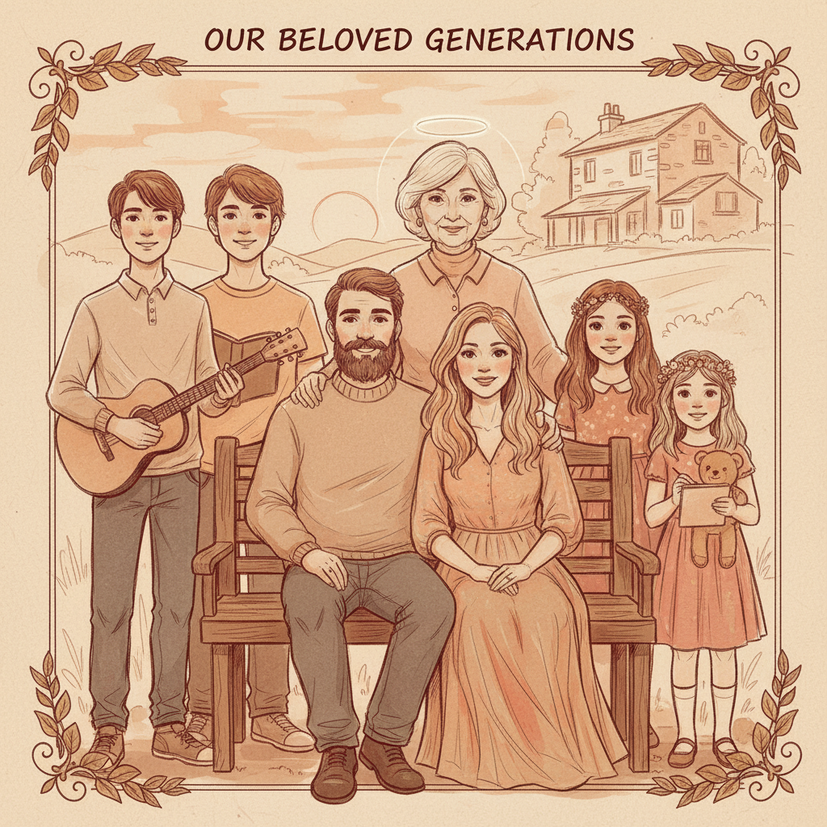
\includegraphics[width=0.85\linewidth]{vokab_300dpi/famill.png} \\
            \vspace{0.3cm}
    }}
    \vspace{0.4em}
    \textbf{\Large D'Famill}\\
    \small\textit{(La famille / The family)}
\end{minipage}
\end{noindent}

\vspace{2em}

\begin{noindent}
\begin{minipage}[t]{0.48\textwidth}
    \centering
    \textbf{\Large Eng Koppel}
    \vspace{0.4em}
    \framebox{\parbox{0.88\linewidth}{\centering
            \vspace{0.3cm}
            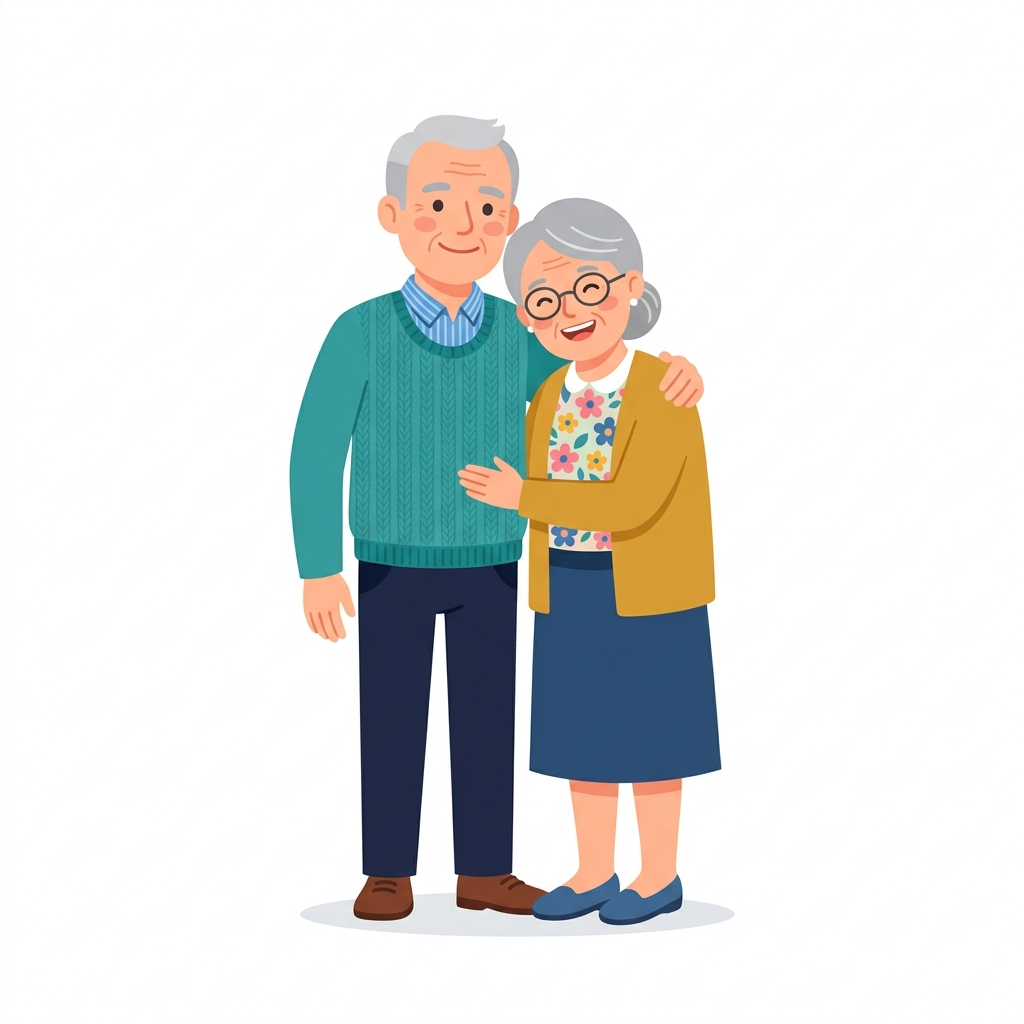
\includegraphics[width=0.85\linewidth]{vokab_300dpi/koppel.png} \\
            \vspace{0.3cm}
    }}
    \vspace{0.4em}
    \textbf{\Large D'Koppel}\\
    \small\textit{(Le couple / The couple)}
\end{minipage}
\hfill
\begin{minipage}[t]{0.48\textwidth}
    \centering
    \textbf{\Large Eng Hochzäit}
    \vspace{0.4em}
    \framebox{\parbox{0.88\linewidth}{\centering
            \vspace{0.3cm}
            
\includegraphics[width=0.85\linewidth]{vokab_300dpi/hochzait.png} \\
            \vspace{0.3cm}
    }}
    \vspace{0.4em}
    \textbf{\Large D'Hochzäit}\\
    \small\textit{(Le mariage, la fête / The wedding)}
\end{minipage}
\end{noindent}

\vspace{2em}

\begin{noindent}
\begin{minipage}[t]{0.48\textwidth}
    \centering
    \textbf{\Large E Paschtouer}
    \vspace{0.4em}
    \framebox{\parbox{0.88\linewidth}{\centering
            \vspace{0.3cm}
            
\includegraphics[width=0.85\linewidth]{vokab_300dpi/paschtouer.png} \\
            \vspace{0.3cm}
    }}
    \vspace{0.4em}
    \textbf{\Large De Paschtouer}\\
    \small\textit{(Le prêtre, curé / The priest)}
\end{minipage}
\hfill
\begin{minipage}[t]{0.48\textwidth}
    \centering
    \textbf{\Large E Haus}
    \vspace{0.4em}
    \framebox{\parbox{0.88\linewidth}{\centering
            \vspace{0.3cm}
            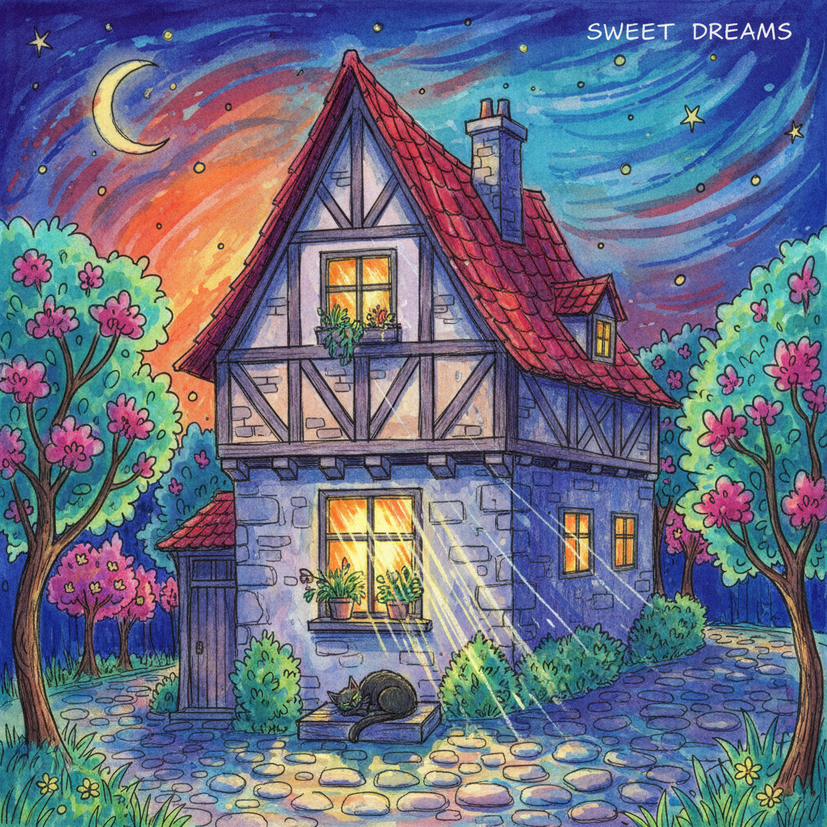
\includegraphics[width=0.85\linewidth]{vokab_300dpi/haus.png} \\
            \vspace{0.3cm}
    }}
    \vspace{0.4em}
    \textbf{\Large D'Haus}\\
    \small\textit{(La maison / The house)}
\end{minipage}
\end{noindent}
